\section{Energetic particles in the heliosphere}
\label{sec:particles_heliosphere}

Introduce all the particles population from lower energy to the higher energy, each population has one paragraph, according to the plot you add, and maybe one plot showed the position of multiple process, could be the plot of blue or the plot in Paddy's thesis



GCR, fully ionized particlesoriginating outside the heliosphere ,accelerated ar supernova remnants [Blasi 2013], covering the energy from typical 1MeV ([Potgieter 2023 LRSP] to ZeV, 90\% of hydrogen, the remain 10\% consist of heavier ions ( percent \%), electron, positron and antiproton (?\%)


The flux , outside the heliosphere,  is isotropic distributed in space and nearly constant in time, while inside of the helioshere, the GCR temporal variaton is highly related with the solar activities and the so-called solar modulation, which are periodcally change in 11 and 22 year period. 






\begin{figure}
	\centering
	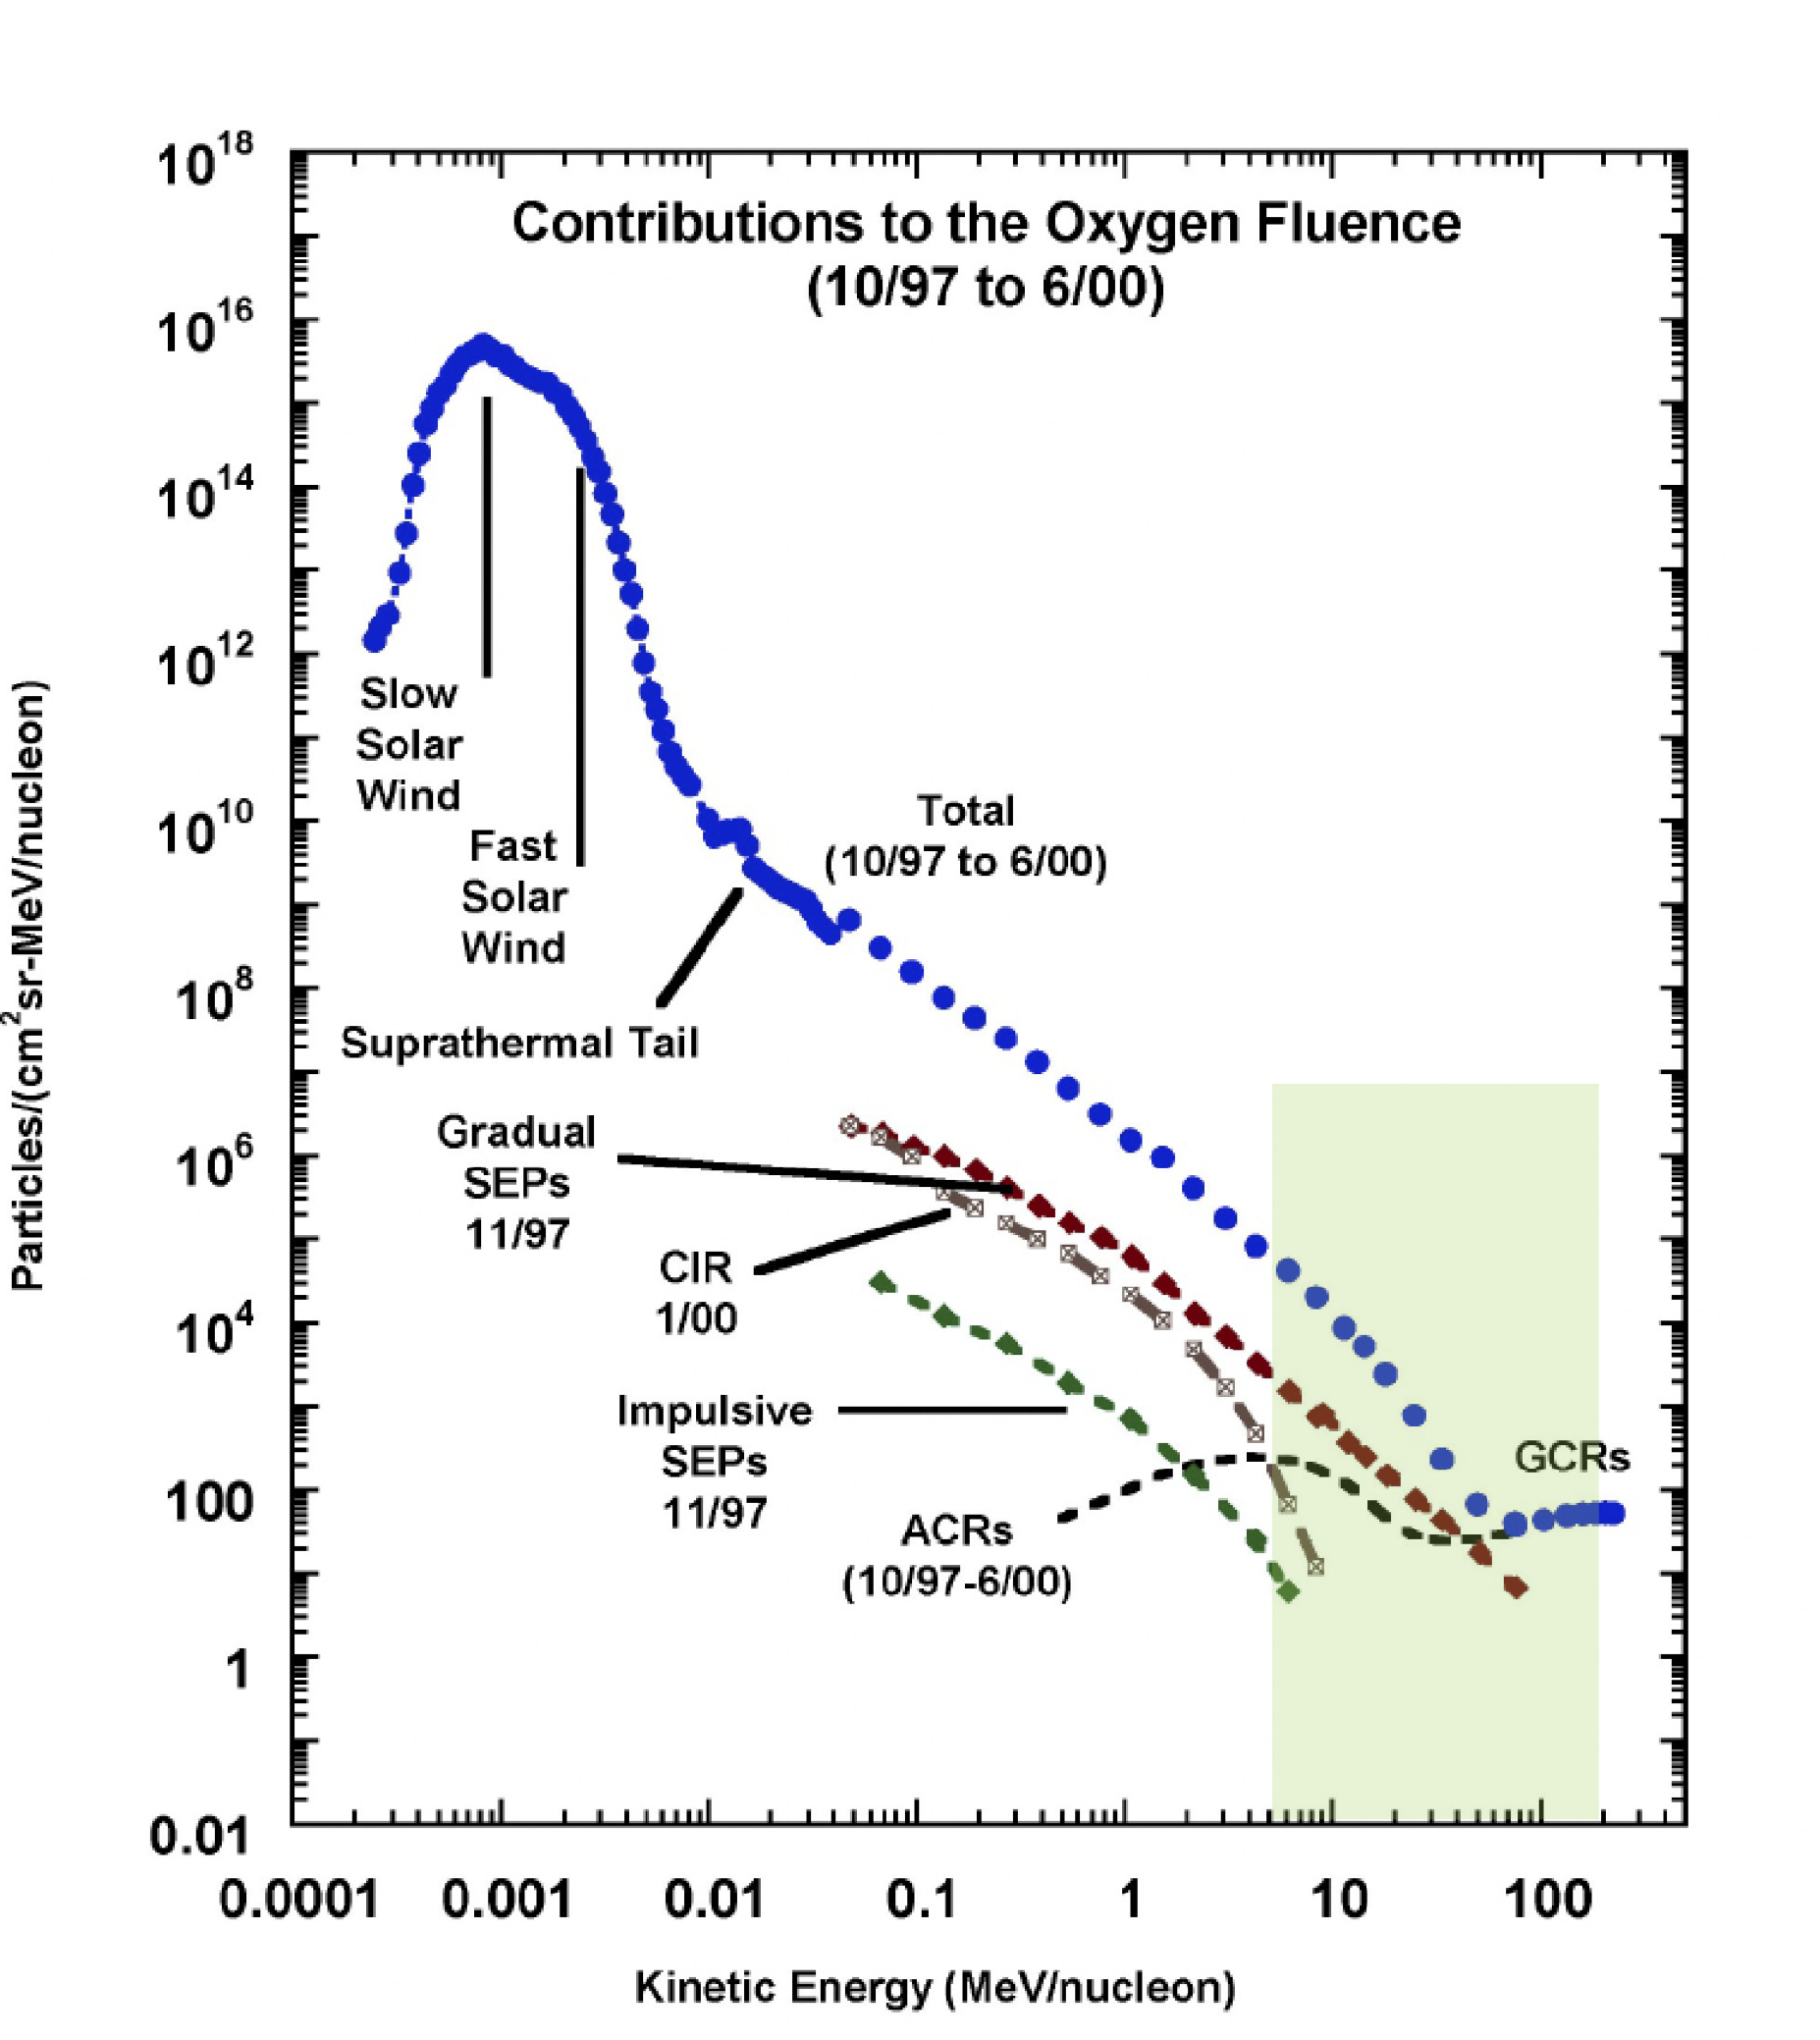
\includegraphics[width = 0.6\textwidth]{images/heliospheric_particle_spectra_color.png}
	\caption[Energy spectra of oxygen ions in the near Earth space]{The typical oxygen spectra in the interplanetary space near the Earth, indicating the contributions of different populations, especially in the energy range between few MeV\/nuc and few hundreds MeV\/nuc, where \acs{SEP}, \acs{ACR} and \acs{GCR} both exist. The spectra of other particles species for instance, helium and proton, have the similar shape but different flux level on corresponding energy region. The figure is adapted from \cite{Mewaldt-2001}}
	\label{Fig:Oxygen_spectra_heliosphere}
\end{figure}

\begin{itemize}
	\item The few tens of MeV energy range is an very important energy range for the heliosphere. In this part the SEP, ACR, lower GCR are bothe there. Therefore, more attention required here
	\item 
\end{itemize}

Our heliosphere is a vast region in space embedded in the \ac{ISM}, which encompasses all solar system planets and extends far beyond even the Kuiper belt. 
It is filled with a thin plasma consisting of various populations of particles, many of which originate from the Sun itself. These populations can be identified in \autoref{fig:heliospheric_energy_spectrum} \citep[based on measurements by][]{Mewaldt-2001}, shown as an energy spectrum that extends over more than 7 orders of 

\section{SEP}

discovery of SEP and history of SEP
- first SEP discovery and the 
\missingfigure[options]{First SEP plot, GLE}
-  Source of SEP at 1980 - flare
 - evidence 1
 - evidence 2
 - most represented result 1
flare math
Two type of SEP and how the source of SEP evolved

Wide spread SEP
	- 
Multi-instrument observation of the SE
The problem of SEP studies



\section{Galactic cosmic rays} ( 1500 words are enough, 50 citation)


The first observation of GCR- Victor Hess, 1912 and he found an electroscope discharged rapidly as he ascended in a ballon.
  (100)
  

GCRs consist of wide range of energetic particles,  which mostly are dominated by the proton, about 89\%  and the remain share are 10\% helium and a small portal of heavier ions (1\%), electron, positron and antiproton. The dominated energy of gcr, as shown in the Fig.\ref{Fig:Oxygen_spectra_heliosphere} is above 100MeV/nuc. Below that, the other component are more common than GCR and it is hard to seperated those particles.

Currently it is believed that those GCR are main originated from the supernova explosion and derived the energy from the shock waves which is genereate from the explosion. When the shock wave travel through the surrounding interstellar gas, the kinetic energy of shock are tranfer to the  (neutral gas?) by the (Fermi-acceleration, ciataion and the acceleration process), Utilimatly, causing the galactic cosmic ray up to 10^12 eV.

Because cosmic rays are fully charged, they are deflected by the magnetic field when they propagation in the interstellar space after speeding up. The directions of those particle are normalized by the strong magnetic field. Hence when they arrived at the local bubble of solar system, we obtained an nearly isotropic and constant intensity profile [citaion of the LSTM,]


To model the solar modulation on the particle transportation of GCR spectra, an input particle spectra need to be specifield, which is the so-call LSTM [ citaion of LSTM]. LSTM is the modulation boundary and will be modulatined as the change of the position, energy, and time after those particle diffusion into the heliosphere. Such a spectra have been observed by the voyeger after then cross the boundary of solar system and enter the interstellar medium
	
A paragraph of local intersteallar spectra


After enter the heliosphere, those high energetic particle are modulated the solar wind and its embedding magnetic field  which change in a 11 year or 22 year period,
The relavant process of the solar modulations could be described by a basic transport equation (TPE) which is first derived by Parker (1965). The same equations was also derived by Gleeson and Axford (1967) in the more rigorous ways. This equation is based on the motion of charged and particle in the high frequently changed magnetic field and averages over the pitch angle of particle moving in the magnetic field. The precondition of this equation is the reasonable assumption of the isotropically distributed GCRs. The TPE give the phase-space distribution function, $f$ as the function of positions, time  and momentum magnetitude. In Potgieter 2013, the helispheric TPE is rewritten in the following form as:

\begin{equation}
	\frac{\partial f}{\partial t} = 

\end{equation}


1. Transport equation( TPE)
	 Parker 1965 derived the basic TPE. More rigorously derivation was carried on by Cleeson and Axford 1967, and the same the function.
	
	add the transport equation and discussion different case
	
    The so-called force field solution is an analyitical solution of the TPE a example of protons
    
    
    With the development of numerical studies, model solution are derived from the transportation model
    Several model like BON14, 2020, CREME and other[Find the paper give the name]. One person  
 the solar cycle and the solar modulation caused change are shown as the the 

\begin{figure}
	\centering
	
	
\end{figure}
	
2 Temperal and spatial variation
	GCR spatial variation
		What is ?
		Why?
		Who first study this topic 
	

3..  temperal variation and GCR solar modulation 
	 The temperal variation comprise of 
	- When the arrived on the local bubble of Solar system- the solar modulation dominate the transport of the particle - General say about 

4.  Interaction of GCR with the planet
	- On the Earth 
		- The process generate the secondary particle
		- Neutron particles	
		
		
	- Interaction with Lunar
	- Interact with Mars 

   


\subsection{ACR}
 1970's found the ACR, by analysie the spectrum of GCR


Both ACR and GCR have the name of cosmic ray, however, if we strictfullyt look at the source, and acceleration process, theACR have the strong heliosphere source rather then the cosmic ray.
Therefore, we seperate the ACR from GCR, though the transport process of those two type of particel in the heliosphere is similar.

Basic observation fact of ACR
- source 

modulation and Transport of Cosmic ray - magnetic field changed with solar activities and affect the transport -  which is reason of the radial gradient change compare to the PSP 

The 
We care about the ACR radial gradient



\subsection{Radiation hazard of energetic particle and the interaction with the planet for instance Moon and Mars}

Radiation hazard of the SEP 
- Space
- on the planetary environment
Radiation from GCR and the secondary particle generated by the GCR

- GCR interaction with regolith, lunar-
	- Generation of Neutron

The exploration of space has witnessed a surge in intensity, with an increasing number of countries aspiring to venture into this domain. Noteworthy examples include NASA's initiation of the Artemis mission, which aims to return to the Moon by 2024. Similarly, China has unveiled its plans to establish a lunar base on the lunar surface by the 2030s, while the European Space Agency (ESA) has also embarked on a lunar lander mission. Most recently, a Japanese lunar lander mission was launched; however, it regrettably encountered failure.

Under these circumstances, the study of solar energetic particles (SEPs) assumes greater significance. SEPs pose a significant radiation hazard for future human exploration on the lunar surface. The most hazardous SEP events have the potential to induce radiation increases of substantial magnitude.

\subsection{Motivition}
New instrument, new data, 
Now observation point.
new solar cycle, special solar Cycle
new solar minimum, special solar minimum





magnitude on the energy scale and about 20 orders of magnitude on the intensity scale.
\begin{figure}
    \centering
    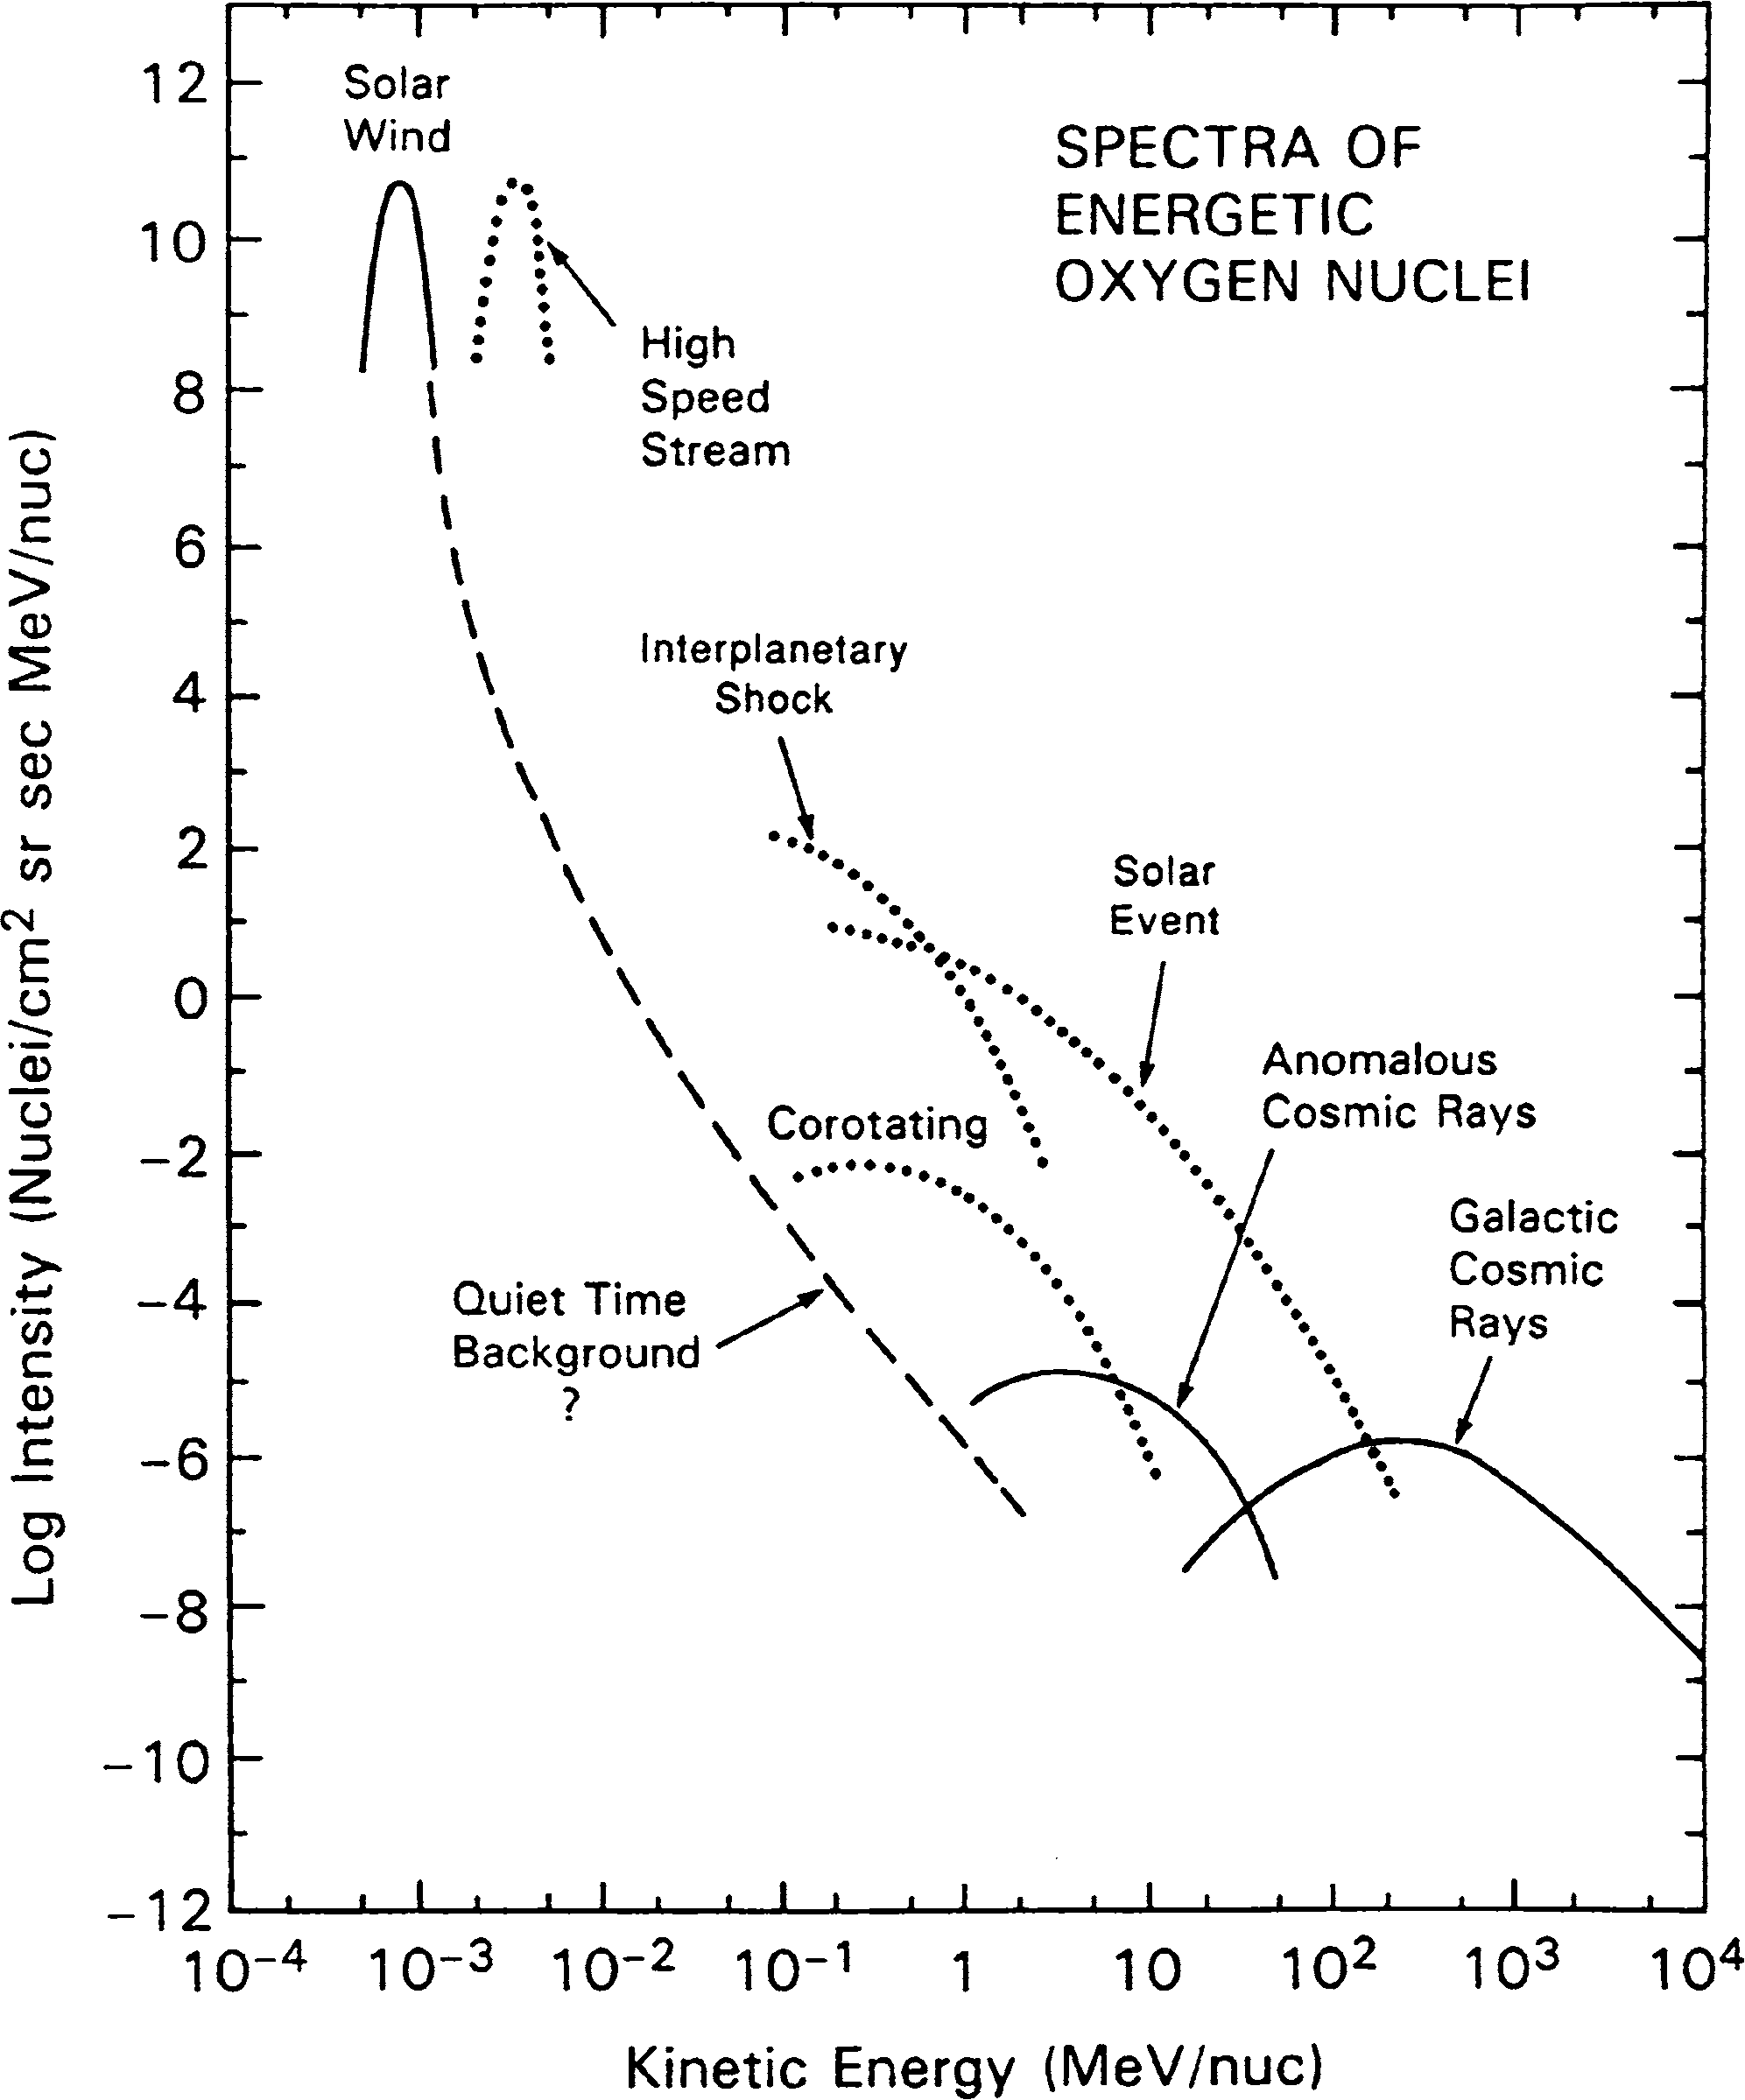
\includegraphics[width=0.6\linewidth]{images/heliospheric_energy_spectrum}
    \caption[Spectra of oxygen ions in the near-Earth interplanetary space]{Typical spectra of oxygen ions in the near-Earth interplanetary space, showing the contributions of different populations. Other particle species show similarly shaped spectra when plotted as a function of energy per nucleon (adapted from \url{http://helios.gsfc.nasa.gov/ace/gallery.html}, based on \cite{Mewaldt-2001}).}
    \label{fig:heliospheric_energy_spectrum}
\end{figure}
